\chapter{Stand der Technik}
\label{cha:technikstand}
Auf dem Markt gibt es eine Vielzahl von Systemen die eine automatisierte XML Schemagenerierung anbieten.
Als Basis zur Generierung gibt es zum Beispiel bestehende Tabellen einer relationalen Datenbank, oder ein bestehendes XML Dokument mit allen möglichen XML-Elementen. Im Folgenden werden die Grundlagen von XML Schema und Schematron erklärt, da diese auch im Konzept von Bedeutung sind.

\section{XML Schema}
\label{cha:Schema}
XML Schema ist eine Sprache zur Beschreibung von XML Dokumenten. Sie bietet eine Vielzahl von Konstrukten um komplexe Strukturen abbilden zu können und die Integrität eines XML Dokuments sicher zu stellen.

\subsection{Aufbau}
Ein XML Schema wird in XML Syntax geschrieben und ist deswegen gut strukturiert und leicht lesbar.
Neben bereits vordefinierten Datentypen für Text, Zahlen und Datum können auch eigene Datentypen definiert werden. Für die Beschreibung des Datentypen kann das \emph{xsd:attribute}-Element verwendet werden. Diese bietet vordefinierte Typen wie \emph{xsd:integer} und \emph{xsd:string}. Mehr dazu in \textcite{Wheeler2011}.

Wie \textcite{Madhavan2001} beschreiben, kann man mit mit XSD eigene Datentypen definieren und diese auch in eigenen Namensräumen deklariert werden. Somit kann jeder Datentyp genau identifiziert werden, und es kommt zu keiner Kollision mit den gewählten Bezeichnungen der Datentypen.
Auch sind Lösungen zur Wiederverwendung von bereits definierten Typen vorhanden. Dies ermöglicht eine bessere Wartbarkeit und verhindert Redundanzen und Fehler in den Beschreibungen.

Dabei unterscheidet man die Datentypen in zwei verschiedene Typen:

\begin{enumerate}
\item \textbf{Einfacher Datentyp}: Wird verwendet um Einschränkungen, Kombination oder Listen von definierten Typen zu realisieren. Die Bezeichnung des Elements lautet \emph{simpleType} (siehe Codebeispiel \ref{fig:simpleTypeExp}).
\item \textbf{Komplexer Datentyp}: Wird verwendet um Sub-Elemente und Attribute zu definieren. Dabei ist auch die Verschachtelung von komplexen Datentypen zulässig. Die Bezeichnung des Elements lautet \emph{complexType} (siehe Codebeispiel \ref{fig:complexTypeExp}).
\end{enumerate}

\begin{program}
\centering
\lstset{
    language=Xml,
    tabsize=3,
    %frame=lines,
    frame=shadowbox,
    rulesepcolor=\color{gray},
    xleftmargin=20pt,
    framexleftmargin=15pt,
    keywordstyle=\color{blue}\bf,
    commentstyle=\color{OliveGreen},
    stringstyle=\color{red},
    numbers=left,
    numberstyle=\tiny,
    numbersep=5pt,
    breaklines=true,
    showstringspaces=false,
    basicstyle=\footnotesize,
    emph={food,name,price},emphstyle={\color{magenta}}}
    \lstinputlisting{images/simpleType.xml}
\caption{Beispiel für \emph{simpleType}}
\label{fig:simpleTypeExp}
\end{program}

\begin{program}
\centering
\lstset{
    language=xml,
    tabsize=3,
    %frame=lines,
    frame=shadowbox,
    rulesepcolor=\color{gray},
    xleftmargin=20pt,
    framexleftmargin=15pt,
    keywordstyle=\color{blue}\bf,
    commentstyle=\color{OliveGreen},
    stringstyle=\color{red},
    numbers=left,
    numberstyle=\tiny,
    numbersep=5pt,
    breaklines=true,
    showstringspaces=false,
    basicstyle=\footnotesize,
    emph={food,name,price},emphstyle={\color{magenta}}}
    \lstinputlisting{images/complexType.xml}
\caption{Beispiel für \emph{complexType}  
}
\label{fig:complexTypeExp}
\end{program}

\subsection{XML Schema 1.1}
\label{section:Schema1_1}
Mit der Version 1.1 des XML Schema sind einige wertvolle Neuerungen dazugekommen. Dazu zählt die Möglichkeit zur Definition von Geschäftsregeln. Dies ist ein sehr ähnlicher Funktionsumfang wie bei Schematron, mehr dazu in Bereich \ref{cha:Schematron}.
Wie \textcite{Walmsley} erläutert, können die dafür notwendigen Annotation direkt bei den jeweiligen Typen ergänzt werden.

Als Beispiel dazu angeführt werden:
\begin{enumerate}
\item \textbf{assert}: Mithilfe von XPath-Ausdrücken (siehe Abschnitt \ref{sec:XPath}) können Bedingungen definiert werden, die zusätzlich die Gültigkeit des XML Elements überprüfen (siehe Codebeispiel \ref{fig:AssertExp}).
\item \textbf{alternative}: Mit \emph{alternative} kann man eine bedingte Typzuordnung realisieren. Dies ist sinnvoll, wenn zum Beispiel sich der Typ aufgrund eines Wertes in einem XML Attribut ergeben soll (siehe Codebeispiel \ref{fig:AlternativeExp}).
\end{enumerate}

\begin{program}
\centering
\lstset{
    language=xml,
    tabsize=3,
    %frame=lines,
    frame=shadowbox,
    rulesepcolor=\color{gray},
    xleftmargin=20pt,
    framexleftmargin=15pt,
    keywordstyle=\color{blue}\bf,
    commentstyle=\color{OliveGreen},
    stringstyle=\color{red},
    numbers=left,
    numberstyle=\tiny,
    numbersep=5pt,
    breaklines=true,
    showstringspaces=false,
    basicstyle=\footnotesize,
    emph={food,name,price},emphstyle={\color{magenta}}}
    \lstinputlisting{images/assert.xml}
\caption{Beispiel für \emph{assert}  
}
\label{fig:AssertExp}
\end{program}


\begin{program}
\centering
\lstset{
    language=xml,
    tabsize=3,
    %frame=lines,
    frame=shadowbox,
    rulesepcolor=\color{gray},
    xleftmargin=20pt,
    framexleftmargin=15pt,
    keywordstyle=\color{blue}\bf,
    commentstyle=\color{OliveGreen},
    stringstyle=\color{red},
    numbers=left,
    numberstyle=\tiny,
    numbersep=5pt,
    breaklines=true,
    showstringspaces=false,
    basicstyle=\footnotesize,
    emph={food,name,price},emphstyle={\color{magenta}}}
    \lstinputlisting{images/alternative.xml}
\caption{Beispiel für \emph{alternative}  %%\cite{ArtikelExp}.
}
\label{fig:AlternativeExp}
\end{program}

\section{XML Schematron}
\label{cha:Schematron}
Schematron ist eine Sprache zur Validierung von XML Dokumenten. Sie wurde 1999 von Rick Jeliffe entwickelt.

\subsection{Vorteile}
Mit Schematron ist es möglich, auch Geschäftslogik in einer XML-Datei abzubilden, siehe ISO Standard 19757-3\nocite{ISO_IEC19757}. Wie  \textcite{Lee2000ComparativeAO} aufzeigen, bietet Schematron einen sehr großen Funktionsumfang, der sehr präzise und kompakt definiert werden kann.
Im Vergleich dazu ist es im XML Schema 1.0 nur möglich auf Datentypen, Bereichswerte oder z.B. auf Referenz-Elemente zu überprüfen, mehr dazu im Bereich \ref{section:Schema1_1}.

\subsection{Funktionsweise}
Beim Schematron können mehrere Geschäftsregeln (engl. \emph{'Business-Rules'}) definiert werden. Diese spiegeln Regeln wider, die den XML-Baum filtern und überprüfen können. Das dafür definierte XML-Element ist 'rule'. Dabei wird zuerst über einen XPath-Ausdruck der XML-Baum gefiltert. Danach können auf diesen XML-Elementen über das 'assert'-Element Testfälle abgefragt werden. Entspricht ein XML-Element dem 'assert' Testfall, so wird dem Benutzer eine dazu zugehörige Fehlermeldung geliefert.
Zu beachten ist, dass sich die Filterungen der 'rule'-Elemente aggregieren und deswegen der Datenbereich immer kleiner wird.
Um wieder vom kompletten XML-Baum zu filtern, muss eine erneute 'Business-Rule' in einem 'pattern'-Element eingeschlossen werden. Mehr dazu in \textcite{Montero2011} Kapitel 5.


\subsection{XPath}
\label{sec:XPath}
XPath ist eine Sprache zur Filterung von XML-Dokumenten. Wie \textcite{Kay2011} beschreibt, wird dabei das XML-Dokument in einer Baumstruktur betrachtet. Jedes XML-Element entspricht einer weiteren Verschachtelung innerhalb des Baumes. Mithilfe von definierten Befehlen kann dann in diesem Baum navigiert und gefiltert werden. XPath ist dabei eine mächtige Sprache und unterstützt eine Vielzahl an Funktionen zur Aggregierung, Quantifizierung und Vergleich der Datenelementen. 

\subsection{Validierung}
Da Schematron mit ISO/IEC 19757-3 standardisiert ist, gibt es die Möglichkeit diese in bestehende Strukturen einzugliedern. Wie \textcite{Akhilesh_validatinga} darstellen, ist es möglich über die XML Elemente \emph{annotation} und \emph{appinfo}, die Schematron-Elemente direkt im XML Schema einzubinden.

\subsection{Transformation}
Die Elemente des Schematron können sehr einfach auf die Elemente einer Extensible Stylesheet Language (XSL) Transformation abgebildet werden.
Dies beschreiben auch \textcite{Tao2013}, die ein Schematron Dokument in ein XSLT Dokument umwandeln. Somit können mögliche Fehler genauer beschrieben und behandelt werden.

\section{SQL-Server}
Als Beispiel genauer betrachtet wird hier die Lösung von \textcite{SqlServer}. Seit SQL Server 2008 unterstützt Microsoft die Generierung von XML Schemata. Dabei ist hier die Generierung nicht auf eine einzige Tabelle beschränkt, sondern kann beliebig über ein SELECT-Befehl angegeben werden. 
Mithilfe des Schlüsselwortes FOR XMLSCHEMA wird aufgrund der ausgewählten Spalten im Ergebnis eine Schema generiert.
Dabei ist auch eine Kombination von Schema und des dazugehörigen XML Dokuments möglich.

Mit dem in Programmcode \ref{code:SqlFORSCHEMA} einfachen SQL-Befehl kann ein gültiges XML Schema erstellt werden. Das Ergebnis, siehe Programmcode \ref{code:GeneratedSchemaSql}, ist ein Schema, das sowohl komplexe, als auch einfach definierte Typen beinhaltet.

\begin{program}
\caption{Beispiel eines SQL-Befehls zur Erstellung eines Schemas}
\label{code:SqlFORSCHEMA}
\begin{GenericCode}
    SELECT ARTIKELNR, QTY
    FROM PRODUKT
    FOR XML AUTO, ELEMENTS, XMLSCHEMA
\end{GenericCode}
\end{program}

\begin{program}
\caption{Generiertes Schema des SQL-Befehls}
\label{code:GeneratedSchemaSql}
\lstset{
    language=Xml,
    tabsize=3,
    %frame=lines,
    frame=shadowbox,
    rulesepcolor=\color{gray},
    xleftmargin=20pt,
    framexleftmargin=15pt,
    keywordstyle=\color{blue}\bf,
    commentstyle=\color{OliveGreen},
    stringstyle=\color{red},
    numbers=left,
    numberstyle=\tiny,
    numbersep=5pt,
    breaklines=true,
    showstringspaces=false,
    basicstyle=\footnotesize,
    emph={food,name,price},emphstyle={\color{magenta}}}
    \lstinputlisting{images/generatedSchema.xml}
\end{program}

\subsection{Vorteile}
Die Generierung der XML Schemata erfolgt sehr performant und ohne zusätzliche Software.
Auch ist es möglich, Felder von mehreren Tabellen zu kombinieren.

\subsection{Nachteile}
Der Datenaufbau bei \BMD ist für den SQL Server oder ähnliche Produkte zu komplex.
Die Einträge in den Tabellen könnten zwar so manipuliert werden, dass diese eine Spalte in dem Ergebnis widerspiegeln, jedoch würde der Datentyp nicht zu dem jeweiligen Feld passen. Hier liegen mehrere Tabellen im Hintergrund, die den Datentypen, die Bereichswerte und die Darstellung im Programm widerspiegeln. 
Gleichzeitig wäre eine explizite Anpassung an mehrere Datenbanksystemen notwendig, da \BMD sowohl Microsoft SQL Server, als auch Oracle unterstützt.

\section{XML Schema aus unstrukturierten Text}
\textcite{Rajbabu2013} zeigen in ihrer Publikation, wie man aus medizinischen Berichte und Kundenbeschwerden  ein XML Schema generieren kann. Dabei analysieren Sie die Texte und erstellen zuerst einen \emph{document object model} (DOM) auf HTML-Tag Basis, siehe Abbildung \ref{fig:DOMobjects}. 

Danach wird der DOM semantisch analysiert und diese Informationen werden als \emph{Semantische Nodes (S-Nodes)} angereichert. Aus dem vollständigen DOM wird danach ein gerichteter azyklischer Graph erstellt. Schlussendlich kann dieser Graph wie ein Stapel abgearbeitet werden, um aus den einzelnen \emph{Nodes} ein XML Schema zu generieren.

\begin{figure}
    \centering
    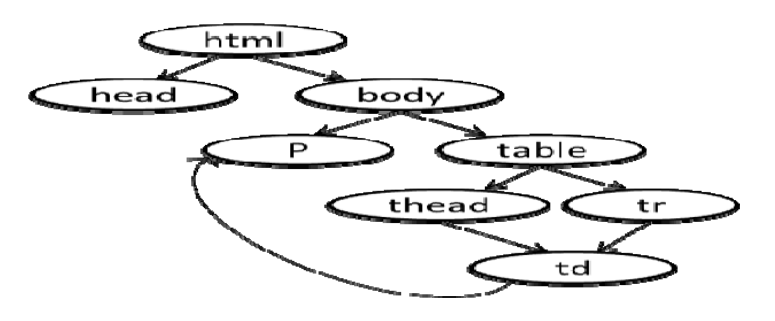
\includegraphics[height=0.5\textheight,width=1\textwidth]{images/domNodes.PNG}
    \caption{DOM-Baum auf HTML Basis, siehe \textcite{Rajbabu2013}}
    \label{fig:DOMobjects}
\end{figure}

\section{Automatische Generierung im medizinischen Bereich}
Auch bei der Umsetzung einer Magisterarbeit von \textcite{Wagner2007} an der TU Wien wurde ein interessanter Lösungsansatz gewählt.
In Zusammenarbeit mit der Krankenanstalt Klagenfurt wurde dabei ein normierter Pflegeentlassungsbericht erstellt. Die Daten wurde dabei in ein Clinical Document Architecture (CDA)-Dokument umgewandelt. Wie man in Programmcode \ref{code:CDA} erkennt, wird ein CDA-Dokument in XML Syntax erfasst.
Wagner zeigt in seiner Arbeit, wie er die Daten klassifiziert und damit ein Datenmodell erzeugt, aus dem schließlich eine XSD-Datei zur Validierung gewonnen werden kann.


\begin{program}
\caption{Auszug eines CDA-Dokument}
\label{code:CDA}
\lstset{
    language=Xml,
    tabsize=3,
    %frame=lines,
    frame=shadowbox,
    rulesepcolor=\color{gray},
    xleftmargin=20pt,
    framexleftmargin=15pt,
    keywordstyle=\color{blue}\bf,
    commentstyle=\color{magenta},
    stringstyle=\color{red},
    numbers=left,
    numberstyle=\tiny,
    numbersep=5pt,
    breaklines=true,
    showstringspaces=false,
    basicstyle=\footnotesize,
    emph={food,name,price},emphstyle={\color{magenta}}}
    \lstinputlisting{images/CDA.xml}
\end{program}

\section{X-Database}
Das Datenmodell X-Database von \textcite{Varlamis2001BridgingXA} zeigt, dass es mithilfe eines XML-Schemas möglich ist, relationale Datenbanken zu generieren und zu manipulieren. Dabei wurden die Datenbank-Befehle in XML-Elementen aufgeteilt. Sie verwenden dabei simple oder komplexe Typen des XML Schema, um daraus Tabellen zu erstellen, siehe Programmcode \ref{code:XmlToSql}. Dabei werden \emph{attribute}-Elemente zur Beschreibung der einzelnen Felder genutzt. 

Auch wird mit Hilfe eines XML Schemas die Struktur von Abfragen und Befehlen auf der Datenbank definiert. Wie man im Programmcode \ref{code:SqlInSchemaForm} sieht, werden Befehle über XML Elemente abgebildet, die zuvor im XML-Schema definiert wurden. Mögliche Befehle sind hier \emph{Insert, Delete, Update} und \emph{Select}.

\begin{program}
\caption{Mapping von XML Schema auf Struktur der Datenbank von \textcite{Varlamis2001BridgingXA}}
\label{code:XmlToSql}
\begin{XmlCode}
<xs:complexType name="DigitalStorageDS">
<xs:attribute name="id" type="ID"
use="required"/>
<xs:attribute name="name" type="string"
use="required"/>
</xs:complexType>
\end{XmlCode}
\label{code:ResultingSQL}
\begin{GenericCode}
CREATE TABLE DigitalStorageDS (
id NUMBER NOT NULL,
name VARCHAR2(20) NOT NULL,
PRIMARY KEY (id));
\end{GenericCode}
\end{program}


\begin{program}
\caption{Auszug eines definierten SQL-Befehls von \textcite{Varlamis2001BridgingXA}}
\label{code:SqlInSchemaForm}
\begin{GenericCode}
    <DBCommand>
    <Select where="@-100@ = 1234">
    <from>
        <AudioVisual id="-96" Name="Gladiator"
         AVType="Movie">
            <MediaInfo id="-97">
            <MediaProfile>
            <MediumRef>-100</MediumRef>
            </MediaProfile>
            </MediaInfo>
        </AudioVisual>
    </from>
    <return>
    <AudioVisualRef>-98</AudioVisualRef>
    </return>
    </Select>
    </DBCommand>
\end{GenericCode}
\end{program}
